\documentclass[11pt,letter]{article}
\usepackage{amssymb}
\usepackage{amsmath}
\usepackage{graphicx}
\usepackage{enumerate}

\addtolength{\oddsidemargin}{-.75in}
\addtolength{\evensidemargin}{-.75in}
\addtolength{\textwidth}{1.5in}
\addtolength{\topmargin}{-.75in}
\addtolength{\textheight}{1.5in}
\setlength{\parindent}{0pt}
\def\bnabla{\mbox{\boldmath$\nabla$}}
\usepackage{subfigure}

\begin{document}
\begin{center}
	\large\textbf{Optimizing Interventions in the Ebola Epidemic Using a Compartmental Model}\\
	\normalsize{Final Report\\APC 524, Fall 2014}
\end{center}

\underline{\textbf{Developers}}\vspace{0.5mm}\\Jesse Ault\\Alta Fang\\Sandra Sowah\\ Yile Gu\\

\underline{\textbf{Project Objective}}\vspace{0.5mm}\\
The software package we propose will determine how to optimally allocate a given, finite number of resources during an Ebola virus outbreak in order to minimize the spread of the disease and contain the outbreak. This software package will use a stochastic compartmental model~[1] to simulate the spread of the disease. Given resource constraints and epidemic information, it will fit the model parameters to the epidemic data and use that model to forecast the effect of certain interventions on the trajectory of the disease. By modeling the effects of different intervention distributions, the software will determine how a fixed quantity of resources can be allocated in order to have the minimal death count due to Ebola epidemic.\\

The software allows user to interact through either a friendly command line interface or a GUI interface. User needs to provide 1) a time series of cumulative Ebola infection case count in a csv file, 2) total population of the corresponding region, and 3) total resources and cost functions for each intervention in a csv file. Then, the program can calculate model parameters, optimal allocation resources, and projections of Ebola spread with or without the allocations (the allocations can be either user specified or the optimal ones from calculations). User has the option to generate figures to inspect the goodness of model fit, as well as the time series of the disease spread. Installation is needed for one part of the code; for details about the installations, please refer to the user manual. 
\\

\underline{\textbf{Compartmental Model Overview}}\vspace{0.5mm}\\

A compartmental model [1-2] has been proposed and used to study the Ebola outbreaks in the Democratic Republic of Congo (1995), in Uganda (2000), and in Sierra Leone and Liberia (2014). In this compartmental model, individuals are classified as: (1) susceptible individuals (S) who can be infected by the Ebola virus following contact with infectious cases; (2) exposed individuals (E) who have been infected by the Ebola virus but are not yet infectious or symptomatic; (3) symptomatic and infectious individuals in the community (I); (4) hospitalized Ebola cases (H) who are infectious; (5) dead Ebola cases (F) who may transmit the disease during funerals; and (6) individuals removed from the chain of transmission (R, cured or dead and buried). The dynamics for the population of these types of individuals are modeled through coupled ordinary differential equations (ODEs) with stochastic components, as shown in Figure~\ref{cmodel} below.\\

\begin{figure}[t]
\centering
\includegraphics[width=8cm]{cmodel.pdf}
\caption{Compartmental model~[1] for Ebola spread.
\label{cmodel}}
\end{figure}


These governing ODEs consider the populations of each compartment to be continuous. However, the populations are rather always discrete as integers. To encounter this problem, the previous studies [1-2] suggested that these simulations could be performed using Gillespie's first reaction method [3]. We implemented the method in C++. Details about the method would be discussed in the section of \underline{Design Process}. \\


Several parameters in the model as in Figure~\ref{cmodel} can be tuned to reflect the levels of prevention or intervention:% as in Table~\ref{para}:

\begin{center}
\centering
%\caption{Model parameters that can be changed through preventions or interventions}
\begin{tabular}{|c|c|c|}
\hline
\textbf{Parameter} & \textbf{Intervention}                                                                       & \textbf{Effect}                                                                                  \\ \hline
$\beta_H$          & \begin{tabular}[c]{@{}c@{}}Personal protective equipment\\  and other supplies\end{tabular} & \begin{tabular}[c]{@{}c@{}}Contact rate for \\ hospitalized cases\end{tabular}                   \\ \hline
$\delta_2$         & Hypothetical drug                                                                           & \begin{tabular}[c]{@{}c@{}}Fatality rate of \\ hospitalized patients\end{tabular}                \\ \hline
$\theta_1$         & \begin{tabular}[c]{@{}c@{}}Contact tracing and \\ community awareness\end{tabular}          & \begin{tabular}[c]{@{}c@{}}Fraction of infected \\ cases diagnosed and hospitalized\end{tabular} \\ \hline
\end{tabular}
\label{para}
\end{center}

In this project, it is assumed that $\beta_H$, $\delta_2$ increases and $\theta_1$ decreases linearly as the resource allocated to each of them increases. Given a fixed quantity of resources, we determine how to most efficiently allocate those resources amongst these three intervention methods to minimize the number of death from the Ebola disease. This is done by incorporating the epidemic model into an optimization cost function and performing constrained optimization to calculate the most efficient resource allocation that will minimize the expected number of deaths.\\

In other words, we minimize $f(x_1,x_2,x_3)$ subjected by the constraint that $\sum\limits_{1}^{3}x_i=1$ and $x_i>0$. $f(x_1,x_2,x_3)$ calculates the expected/averaged number of deaths corresponding to a given allocation of resources by running the stochastic simulations with many trajectories. $x_i$ represents the fraction of total resource allocated to each of the three interventions. \\

\underline{\textbf{Tools Used}}\vspace{-0.5mm}\\

The tools used in this project are shown below:


\begin{center}
\centering
       %   \caption{Tools used in this project.}
	\begin{tabular}{ l | p{13cm}}
           \textbf{Purpose} & \textbf{Tool or resources} \\ \hline
	Visualization in Python & Matlplotlib \\
	Optimization in Python & Scipy \\
	Documentation  & Sphinx \\
	Documentation  & Sphinx \\
         Testing  & Python Unittest \\
         Coupling between C++ and Python & Cython \\
         Version Control & Git \\
         Profiling & Not sure 
         
	\end{tabular}
%	\label{tool}
\end{center}

\underline{\textbf{Design Process}}\vspace{0.5mm}\\

Except for the part where Gillespie\rq{}s first reaction method is implemented in C++, all the implementation is performed in Python. Figure~\ref{UML} is the UML (unified modeling language) of the code.
\begin{figure}[h]
\centering
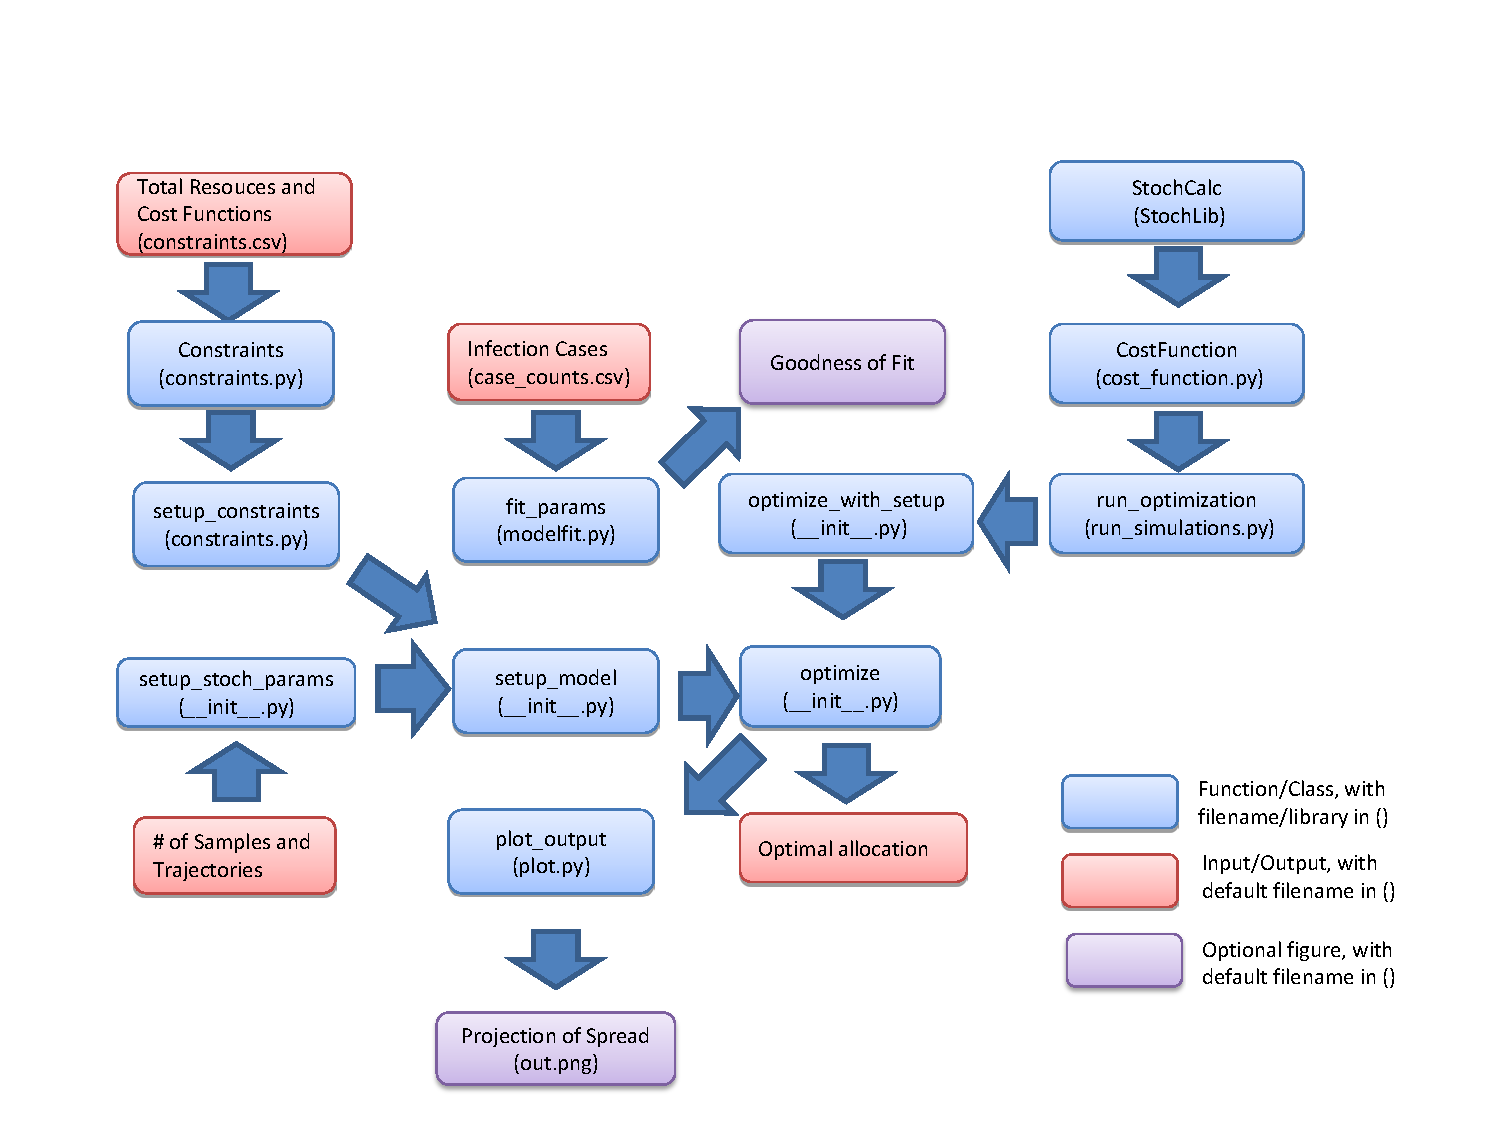
\includegraphics[width=16cm]{Design_FlowChart.pdf}
\caption{UML of the code
\label{UML}}
\end{figure}\vspace{-2mm}

Several major functions in this UML are discussed below.

\begin{itemize}
  \item fit\_params
  
 \emph{Functionality:} 
 In this function, inputs are the data of infection cases and respective population, and the outputs are the model parameters and optionally a figure comparing the data with the model.
  
 \emph{Specifics:} 
 A deterministic version of the compartment model is implemented as a function named SIRode. The model parameters are initialized using the values from literature [2]. COBYLA method from Scipy is used to minimize the difference between the model predictions and data, with appropriate constraints on model parameters. The model parameters calculated are then stored in the object OrigParams, which is then used in other functions. 

  \item StochCalc
  
   \emph{Functionality:} 
   Gillespie's first reaction method [3] is implemented which calculates many trajectories. For each trajectory, time series of population in each compartment is obtained. According to the Gillespie algorithm [3], for each trajectory, the following steps are followed:
     \begin{itemize}
       \item 1. Initialize the populations and reaction constants.
       \item 2. For each possible reaction, calculate the probability it will be the next reaction.
       \item 3. Generate random numbers to determine the next reaction using the probabilities and the time interval.
       \item 4. Update and repeat until the final time.
     \end{itemize}
 \emph{Specifics:} 
C++ solver written to utilize only the Gillespie algorithm for the specific rate equations of our compartmental model. OpenMP is included to allow the user to optionally run the code on parallel. Cython is used to call the C++ StochCalc solver from our Python optimization loop. Two classes are used to hold all the parameters for the solver as shown in Figure~\ref{cython}. Python equivalent classes are passed between the Python and C++ codes.

\begin{figure}[h]
\centering
\includegraphics[width=16cm]{cython.pdf}
\caption{Two classes that hold all the parameters for the solver in C++
\label{cython}}
\end{figure}

  \item run\_optimization
  
   \emph{Functionality:} 
  This function uses the model parameters obtained from fit\_params, and utilizes StochCalc to determine the expected/averaged number of deaths. Through optimization, it finds the optimal allocation.
  
 \emph{Specifics:} 
 COBYLA method from Scipy is used for minimization. The function to be minimized is represented by a class CostFunction which calls StochCalc for calculations and initializes itself using parameters from fit\_params as well as user input. To prevent unreasonable results, two things are checked before performing the optimizations. Specifically, the prevention time is checked to make sure that the prevention time is greater than the final time of the history data. Also, the total resource is checked to ensure that it is not too much such that all the three interventions can all be maximized. Optimization is not needed if either of these cases is invalid. 
\end{itemize}

\underline{\textbf{Testing}}\vspace{0.5mm}\\

Unitest is used to test python scripts. All the test files are included in \emph{tests} folder under \emph{ebolaopt} folder. \\

\emph{test\_modelfit.py} is used to test function \emph{fit\_params}. 

\begin{itemize}

\item \underline{test1:} It tests that the code gives reasonable results for different countries.
\item \underline{test2:} It tests that the code can optionally gives figures comparing model predictions with history data.

\end{itemize}

\emph{test\_optimization.py} is used to test resource allocations.
\begin{itemize}

\item \underline{test1:} It tests that the optimization would not run if the prevention time is after the final time.
\item \underline{test2:} It tests that the optimization would not run if too much total resource is present.
\item \underline{test3:} It tests that the optimization would work for different countries.
\item \underline{test4:} It tests that the boundary cases where all the resources is allocated to one particular prevention.
\item \underline{test5:} It tests that the parallelization capabilities of the code.
\item \underline{test6:} It tests that the optimal resource allocations obtained from the code here actually give better results than non-optimal resource allocations. More details about the results from this test are included in the section \underline{Simulation Results and Discussions}.
\end{itemize}

\underline{\textbf{Profiling}}\vspace{0.5mm}\\

Gillespie's first reaction method is identified as the most computationally intense part of the code. To speed up this part of the code, the method is written in a problem specific C++ code, rather than using StochPy, a generic Python tool. As shown in table below as well as in Figure~\ref{speed_up}, significant speed-up can be achieved by choosing StochCalc, the C++ code written in this project, over StochPy. For both StochCalc and StochPy, the required run time increases linearly with the number of trajectories. \\

 \begin{figure}[t]
\centering
\includegraphics[width=16cm]{speed_up.pdf}
\caption{Comparsons of the run time of the Gillespie's first reaction method between StochPy and StochCalc for various numbers of trajectories.
\label{speed_up}}
\end{figure}

\underline{\textbf{Simulation Results and Discussions}}\vspace{0.5mm}\\

To demonstrate the usage of the software, we did a comprehensive study on the recent outbreak in the country of Sierra Leone (test6 in \emph{test\_optimization.py}). The data are obtained from Caitlin Rivers from Virgina Tech, who procure them from World Health Organization and WHO situation reports. \\

As demonstrated in Figure~\ref{model_fit}, the software is able to find the model parameters that fit the data well. 
\begin{figure}
	\centering
	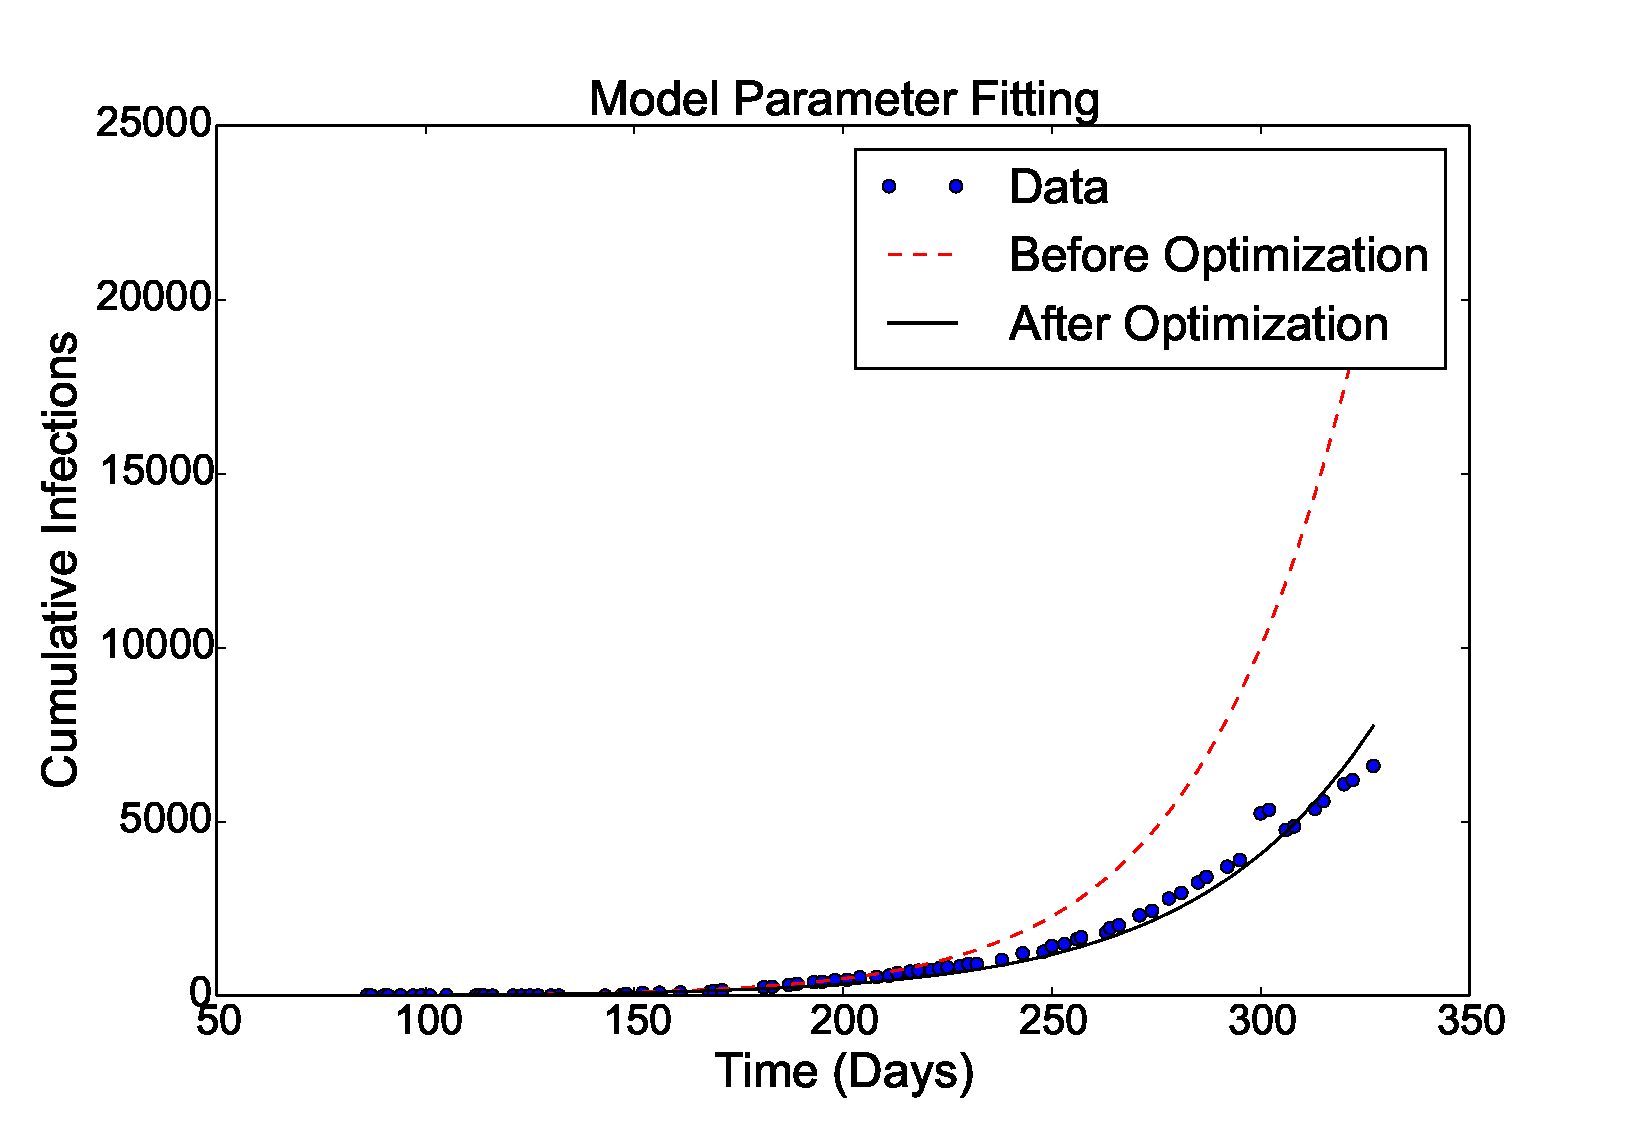
\includegraphics[width = 3.5 in]{model_fit.eps}
\caption{After optimization, the software is able to find model parameters within constraints that improve the model fit with the data for cumulative infections in Sierra Leone.
	\label{model_fit}}
\end{figure}
In order to correctly calculate the optimal resource allocation to minimize number of deaths, the cost of resources for each of the three intervention parameters $\beta_H$, $\delta_2$ and $\theta_1$ needs to be obtained. However, despite much literature research, no concrete information on the subject is found. Here, we assume that:
\begin{itemize}
\item For every $60$ units of resource spent, $\beta_H$ is decreased by $0.01$.
\item For every $500$ units of resource spent, $\delta_2$ is decreased by $0.05$.
\item For every $200$ units of resource spend, $\theta_1$ is increased by $0.01$.
\item We have $10000$ units of resource in total for allocation.
\item The intervention starts at 200 days after the outbreak.
\end{itemize}

From the assumptions above, the software is able to find the optimal resource allocation. The model predictions of Ebola infections over time without and with interventions are shown in Figure~\ref{allocation}(a). As shown in the figure, without the interventions, the infections grow exponentially. People in the Suspect compartment which represents the people who are free from Ebola decrease with increasing speed. With the interventions which start at the day of $200$, the infections are checked and even decrease over time. People who are free from Ebola decrease with much lower speed in comparison. \\

To demonstrate the fact that the optimal resource allocation obtained from this software is indeed a favorable option, we use the same amount of resources but allocate all of them to $\beta_H$, and perform the same calculations to find the Ebola spread over time. The results are shown in Figure~\ref{allocation}(b). After comparison between Figure~\ref{allocation}(b) with Figure~\ref{allocation}(a), it is shown that with the optimal resource allocation, there are less infection cases over time. More people would be free from Ebola. Thus, the optimal resource allocation calculated is indeed an effective allocation. \\
\begin{figure}
	\centering
	\subfigure[]{
	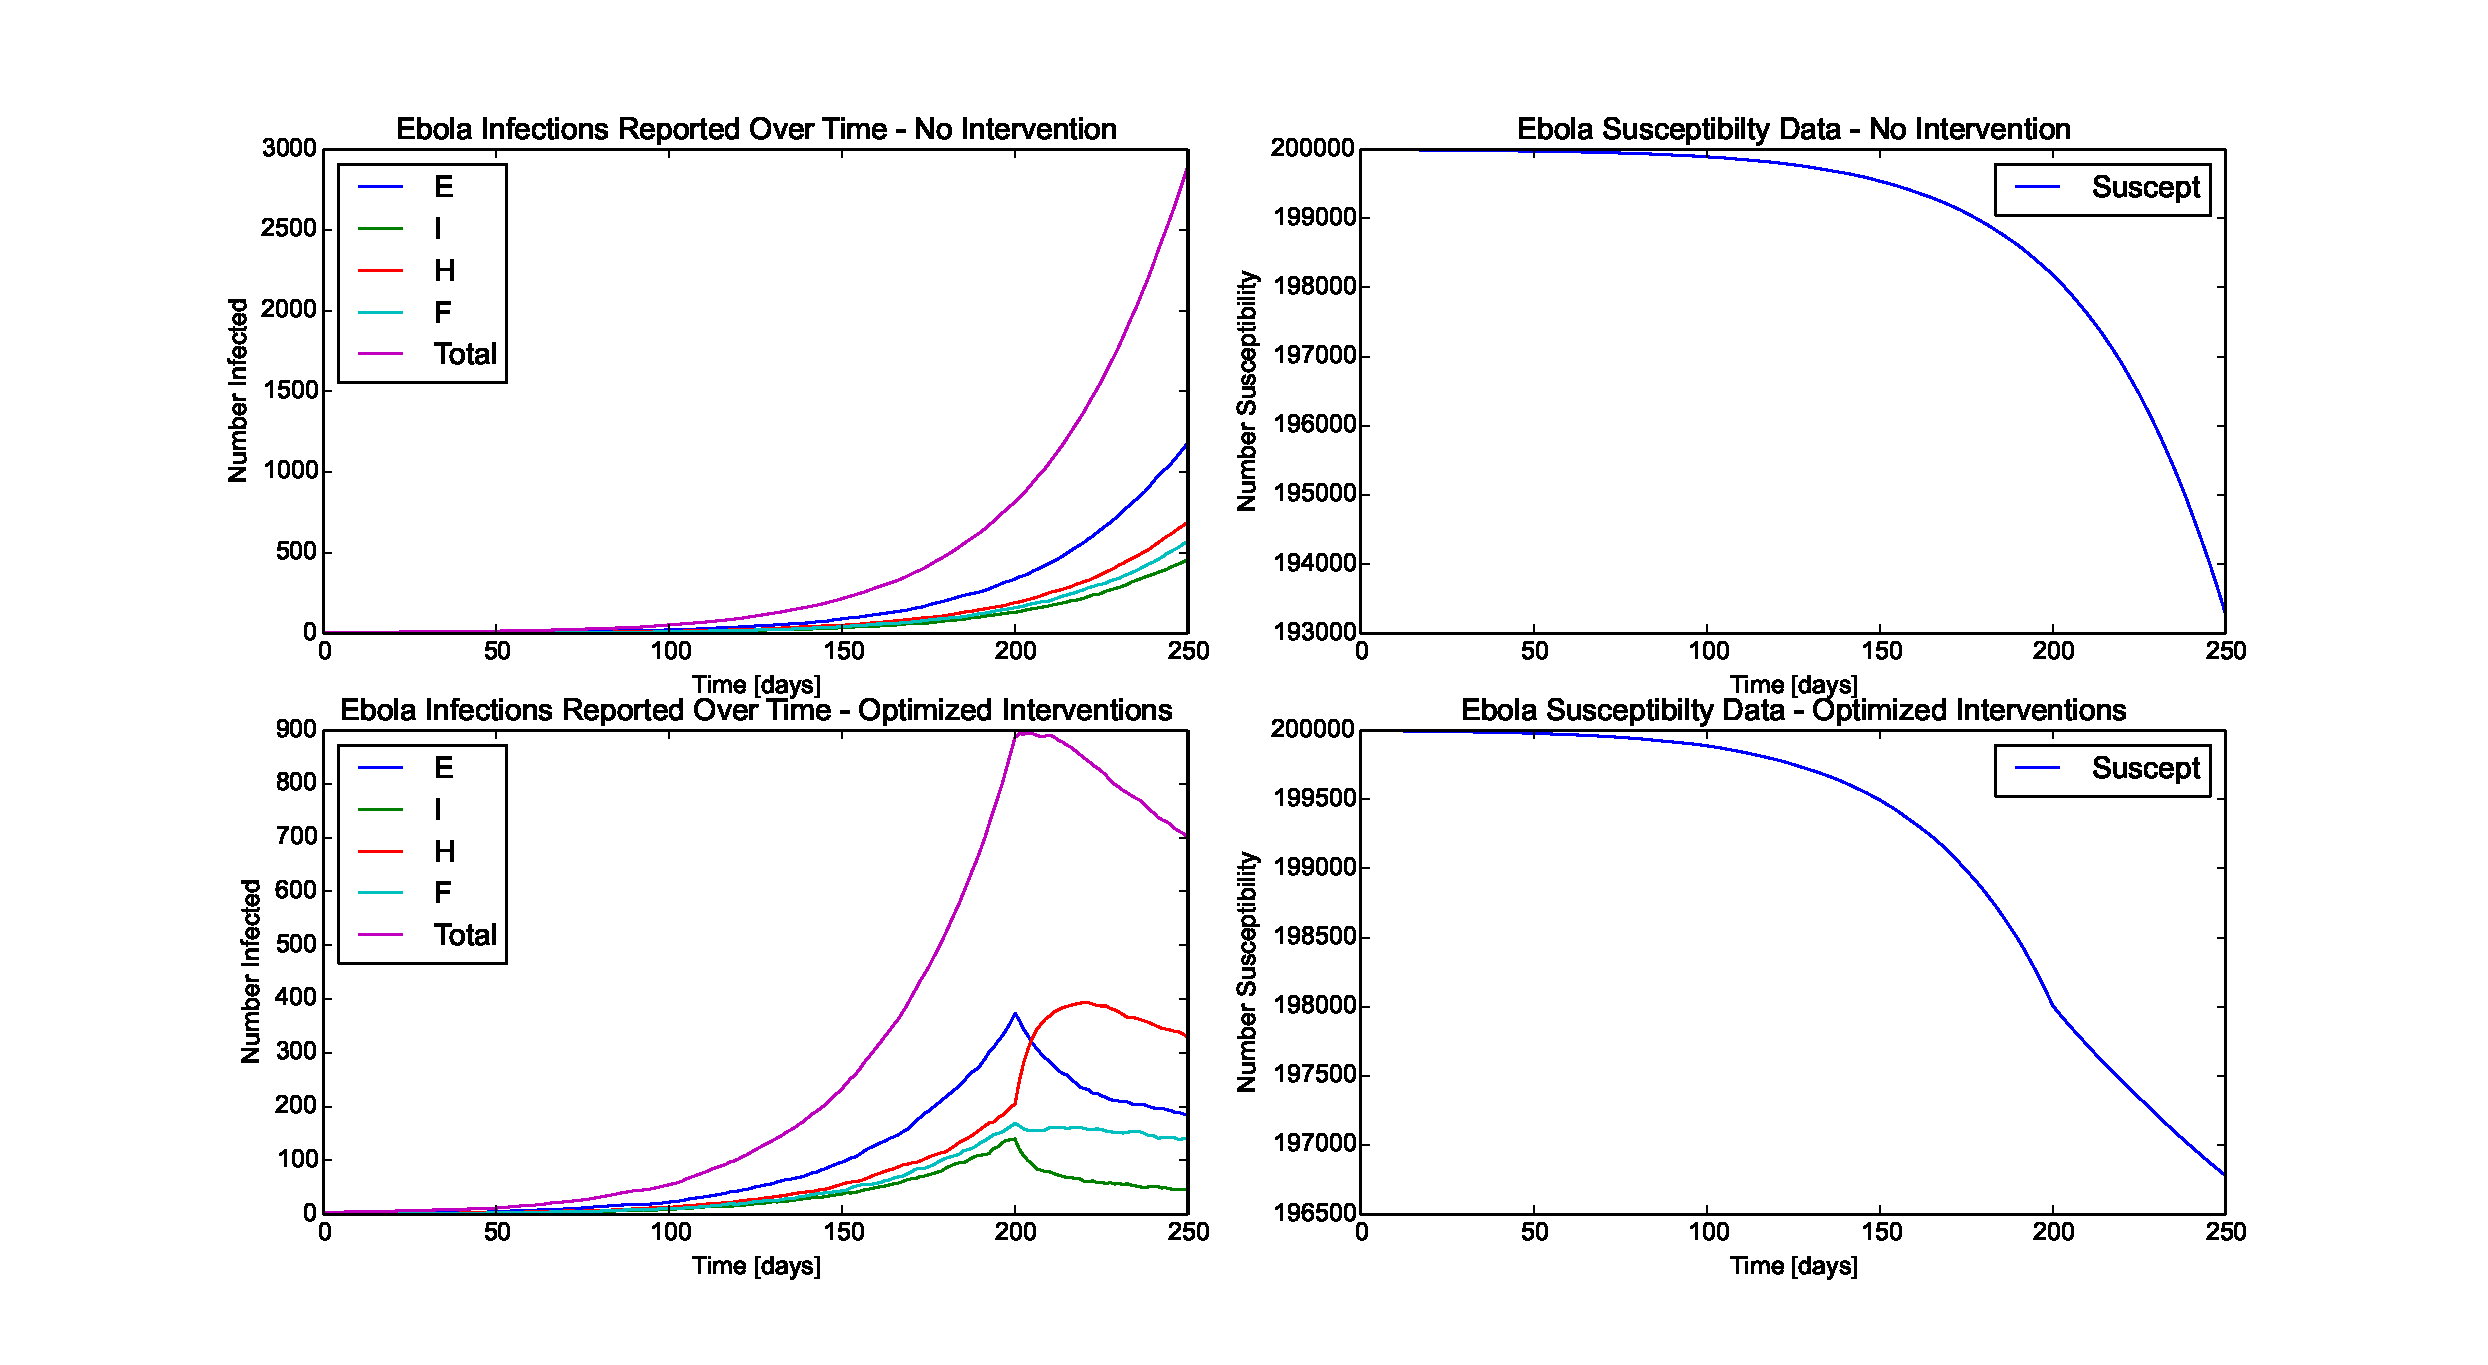
\includegraphics[width = 7.0 in]{optimal.eps}}
	\subfigure[]{
	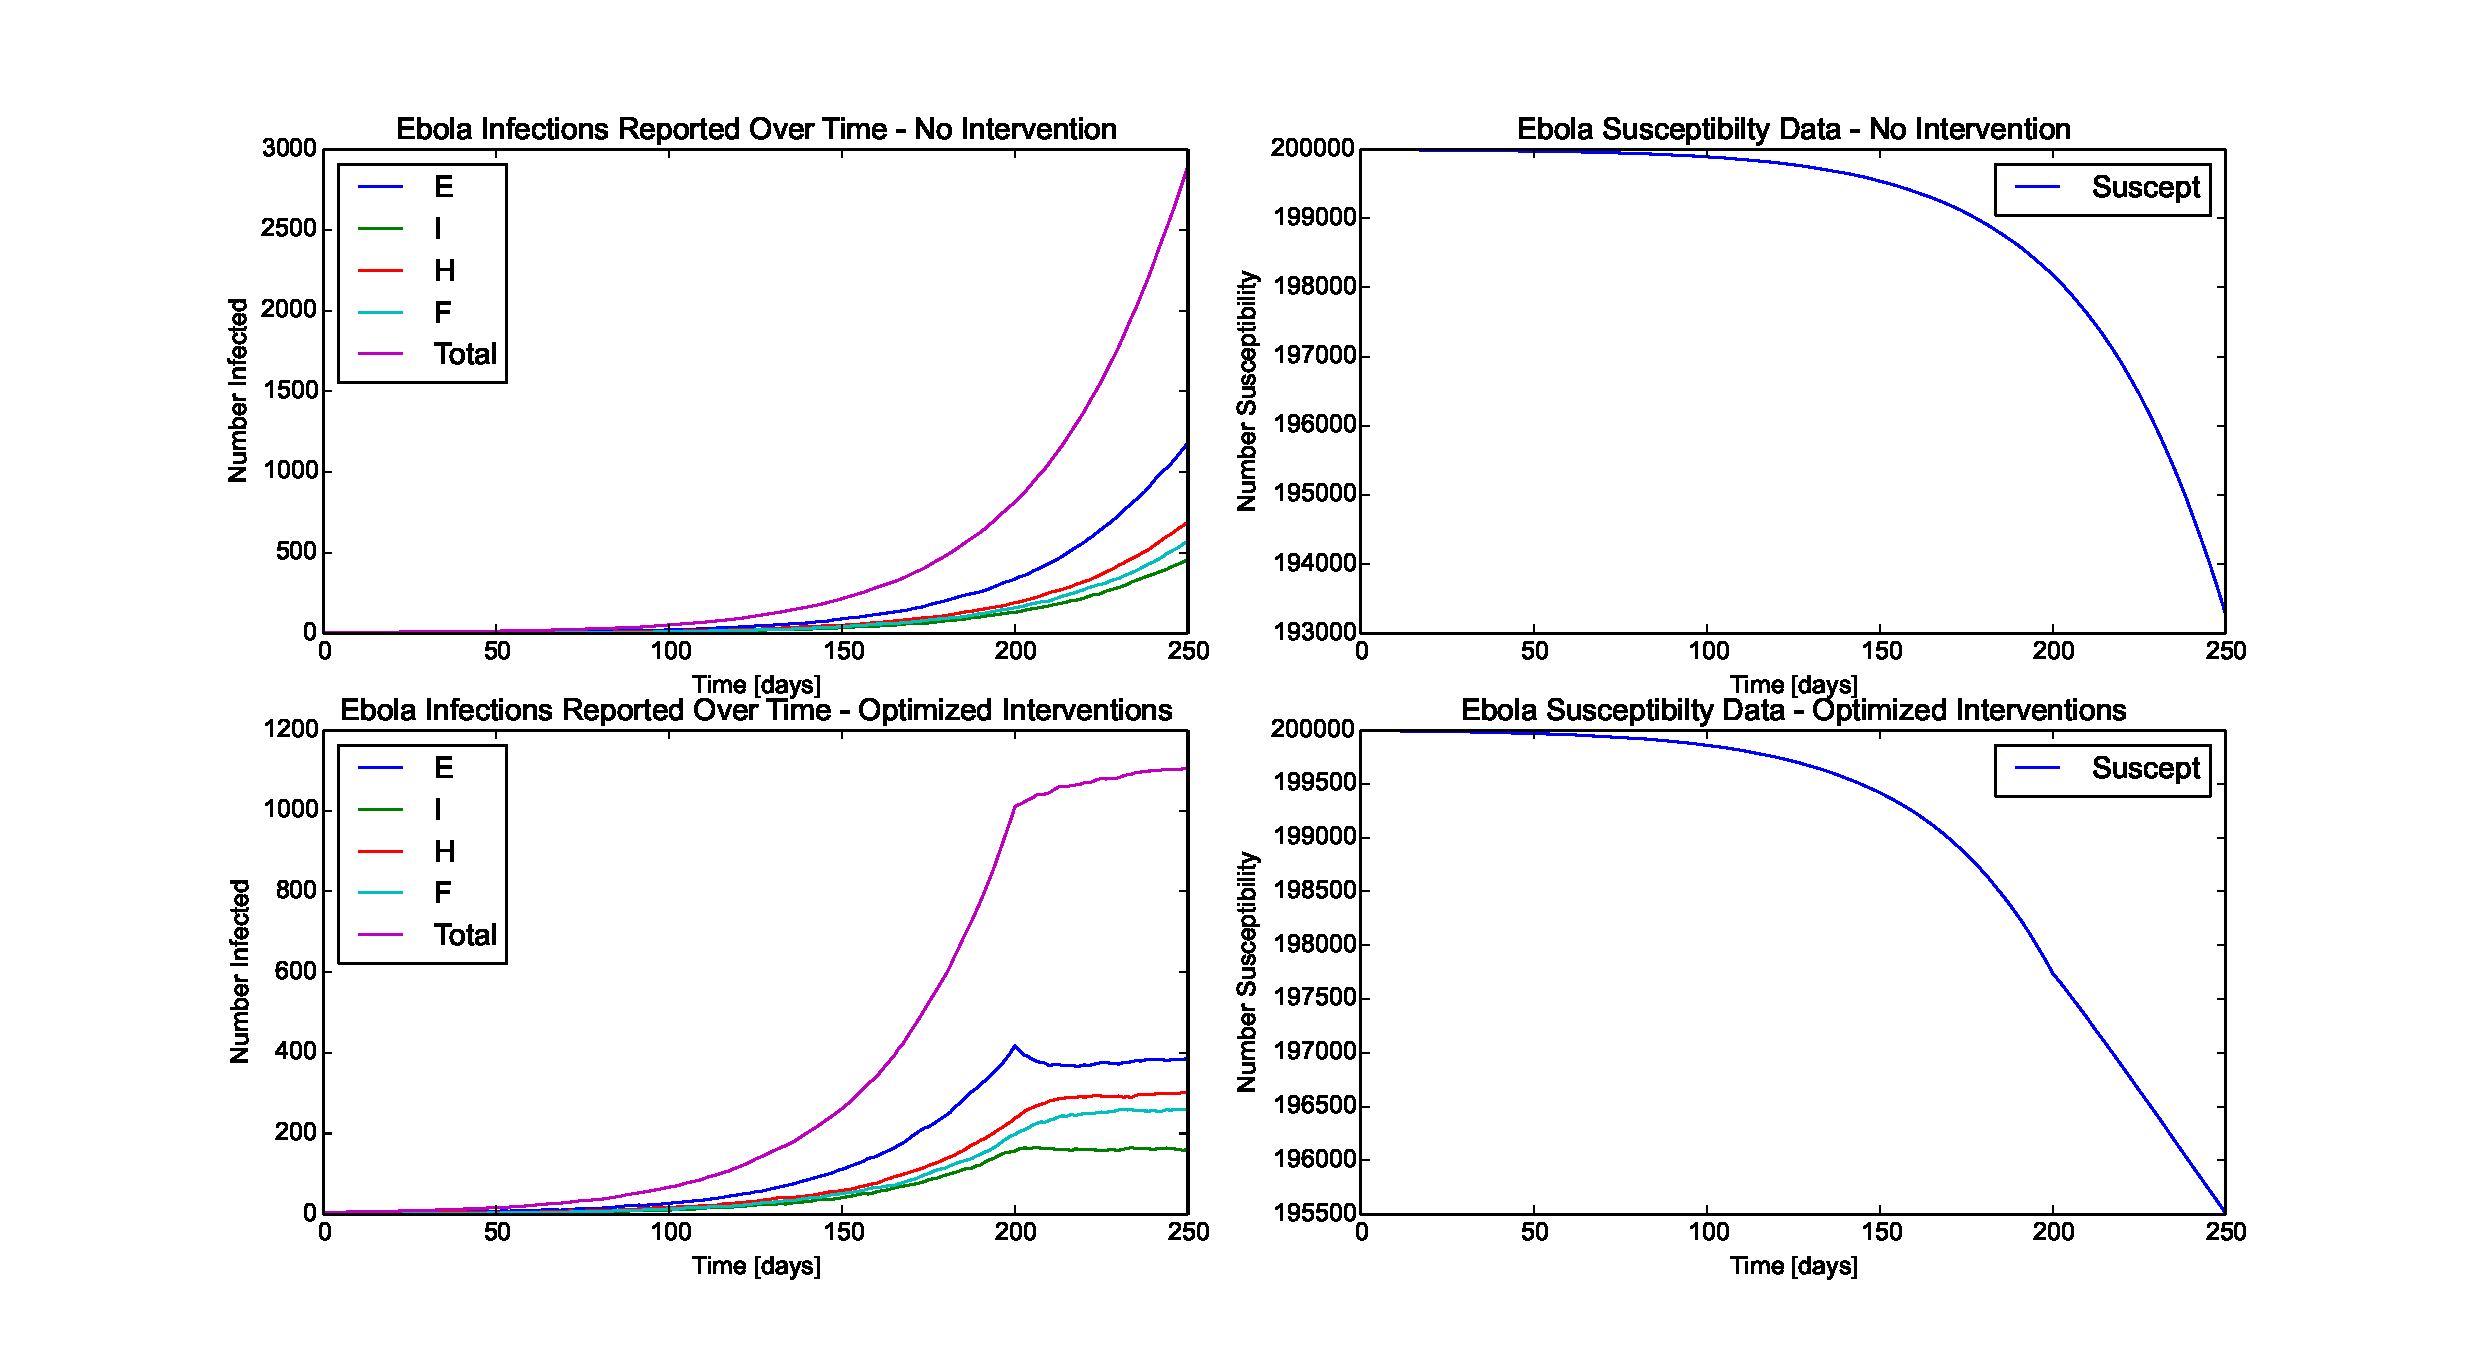
\includegraphics[width = 7.0 in]{not_optimal.eps}}

\caption{
Comparison of Ebola spread over time between the case with no intervention and the one with intervention. In (a), the optimal resource allocation is used. In (b), all the resources is spent on $\beta_H$. 
	\label{allocation}}
\end{figure}


%Development will begin in Python in order to take advantage of the stochastic simulation tool StochPy [4]. After profiling our code, we may translate some of the computationally intensive work of the code into C++, if doing so will be expedient and worthwhile. The majority of the software we develop will focus on generating the initial raw data input in the initial calculation steps and then optimizing the raw data input, taking into account monetary resource allocation for the intervention procedures (in the second stage of re-analysis). Part of our software development will include generating code to interface with StochPy in order to solve a stochastic model for our program. StochPy will be the available off-the-shelf software that our software package will interface with in order to solve the disease model with optimized weighting functions for the optimal monetary resource allocation. SciPy will also be utilized to solve the deterministic ODEs and to solve the least squares minimization problem which will output parameters governing the stochastic equations, which will in turn be used by StochPy. The accuracy of these solutions can be verified by comparing the model parameters obtained in this study with those found in the existing literature [2].\\\\

%\underline{\textbf{User Interface}}\vspace{0.5mm}\\
%A well-documented and clear user interface will allow the compartmental epidemic model to be run easily without the user needing to worry about the details of the implementation (unless they want to). Users will simply input the total amount of available resources, along with various parameters related to the current outbreak, and the software will output predictions of the future of the outbreak, including a total number of infections, based upon different allocations of the resources among the various interventions. No knowledge of disease modeling or the mathematical methods involved will be required by the user!\\

%\textbf{Inputs:}
%\begin{itemize}
%	\item{Raw data of the epidemic trajectory (e.g. historical data containing the number of infections vs. time) so that the software can determine model parameters by fitting to this data. The software will also have some default values if the users want to skip this step.}
%	\item{The fixed resources (e.g. money) dedicated to controlling the epidemic.}
%	\item{Additional constraints, such as which types of interventions are possible or ranges for various parameter values.}
%	\item{The costs of various interventions. The software will also have a default value for these costs.}
%	\item{The user can also choose a format for the output results.}
%\end{itemize}

%\textbf{Outputs:}
%\begin{itemize}
%	\item{The optimal resource allocation (how to allocate the money/personnel over different intervention techniques) that will minimize the total infections over the duration of the outbreak.}
%	\item{The software will also output and optionally plot the effects of particular interventions in order to help the user identify trends in how to achieve the optimum intervention allocation.}
%\end{itemize}



\underline{\textbf{Lessons Learned from the Project}}\vspace{0.5mm}\\

The project gave us an opportunity to experience writing a relatively large code as a team. From the project, we realized the importance of writing a code with good modularity. We also got to practice using github to put the codes together. In addition, we learned to think from the perspective of user when writing the code. This project also gave us a fresh look at how software could help solve important real-world problems. \\


\underline{\textbf{Distribution of Labor}}\vspace{0.5mm}\\
\begin{center}
	\begin{tabular}{ l | p{13cm}}
           Developer & Primary Responsibility \\ \hline
	Jesse Ault & Utilize StochPy to solve the stochastic differential equations that model the Ebola outbreak. \\
	Alta Fang & Wrap the optimization around the stochastic solver and handle user inputs. \\
	Sandra Sowah & Analyze outputs from the StochPy simulations as well as from the optimization, visualize them, and generate outputs for the user. Main contributor to the documentation.\\
	Yile Gu & Fit the raw data of an epidemic's history to a deterministic version of the model in order to generate model parameters which govern the stochastic equations. Main contributor to the final report.
	\end{tabular}
\end{center}

\underline{\textbf{References}}\vspace{0.5mm}
\begin{enumerate}[ {[}1{]} ]
\item{Legrand et al. ``Understanding the dynamics of Ebola epidemics'' Epidemiol. Infect. (2007)}
\item{Rivers et al. ``Modeling the impact of interventions on an Epidemic of Ebola in Sierra Leone and Liberia'' (2014)}
\item{Gillepsie DT. ``A general method for numerically simulating the stochastic time evolution of coupled chemical reactions''. Journal of Computational Physics (1976)}
%\item{Maarleveld. ``StochPy: a comprehensive, user-friendly tool for simulating stochastic biological processes''. PLoS One (2013)}
%\item{http://en.wikipedia.org/wiki/Compartmental\_models\_in\_epidmiology}
\end{enumerate}
\end{document}